\chapter{Porównanie implementacji klasycznych i kwantowej}
\label{chap:combined_results}

W niniejszym rozdziale porównano wyniki wszystkich sprawdzanych implementacji algorytmu Dijkstry: wersji naiwnej, wersji wykorzystującej kopiec binarny oraz wersji kwantowej. 

\section{Porównanie średniej liczby operacji}

\begin{figure}[H]
    \centering
    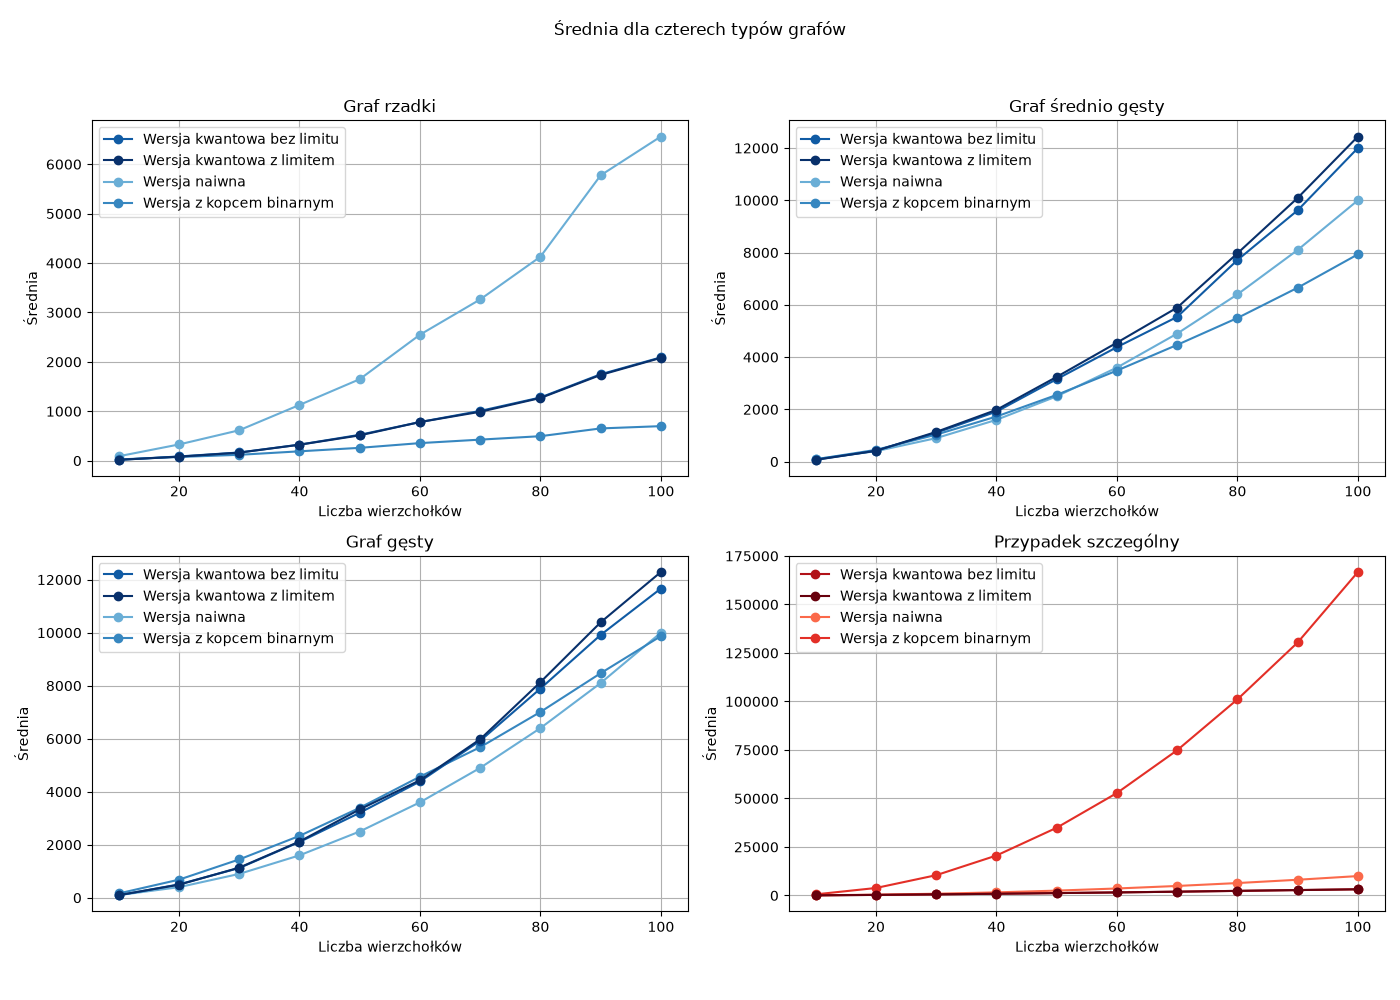
\includegraphics[width=\columnwidth]{images/documentation/combined/combined_mean.png}
    \caption{Porównanie średniej liczby operacji wszystkich badanych implementacji dla czterech typów grafów.}
    \label{fig:combined_mean}
\end{figure}

Na rys.~\ref{fig:combined_mean} przedstawiono porównanie średniej liczby operacji wszystkich badanych wersji algorytmu Dijkstry. Najważniejszą obserwacją jest brak jednej implementacji, która zachowywałaby się najlepiej dla każdego rodzaju grafu. 

\subsection{Graf rzadki}

Dla grafów rzadkich średnia liczba operacji dla implementacji wykorzystującej kopiec binarny rośnie wyraźnie wolniej niż w przypadku pozostałych metod. Wynika to z niewielkiej liczby krawędzi, która ogranicza liczbę relaksacji oraz liczbę operacji wykonywanych w kopcu. Wersja naiwna zachowuje się gorzej, ponieważ podczas kolejnych wyborów minimum algorytm nadal sprawdza wszystkie wierzchołki. Wyniki wersji kwantowych znajdują się pomiędzy implementacją naiwną a kopcową.

\subsection{Graf o średniej gęstości}

Dla grafów o średniej gęstości różnice pomiędzy implementacjami są mniejsze niż dla grafów rzadkich. Jednak wraz ze wzrostem liczby wierzchołków różnice te się powiększają. Wersja z kopcem nadal lepiej wykorzystuje strukturę grafu niż wersja naiwna, ale jej przewaga jest mniejsza niż w przypadku grafów rzadkich ponieważ zwiększenie liczby krawędzi prowadzi do większej liczby relaksacji. Wersje kwantowe wykazują podobny do siebie przebieg a ich koszt rośnie szybciej niż koszt wersji z kopcem. 

\subsection{Graf gęsty}

W przypadku grafów gęstych różnice pomiędzy metodami klasycznymi stają się mniejsze. Rosnąca liczba krawędzi powoduje zwiększenie liczby relaksacji, przez co kopiec stopniowo traci przewagę nad wersję naiwną widoczną dla grafów rzadkich. Wersje kwantowe również wykazują wyraźny wzrost średniej liczby operacji wraz z rozmiarem grafu. Dla większych grafów ich koszt zaczyna być wyższy niż dla wersji klasycznych. 

\subsection{Przypadek szczególny}

Najbardziej wyróżniające się wyniki występują dla przypadku szczególnego. W wersja wykorzystującej kopiec binarny następuje bardzo szybki wzrost liczby operacji podczas gdy średni koszt pozostałych wersji pozostaje niewielki. Przyczyną jest specjalna konstrukcja wag wymuszająca maksymalną liczbę relaksacji. Mechanizm ten został dokładnie opisany w rozdziale~\ref{subsec:special_case_heap_results}.

\section{Porównanie odchylenia standardowego}

\begin{figure}[H]
    \centering
    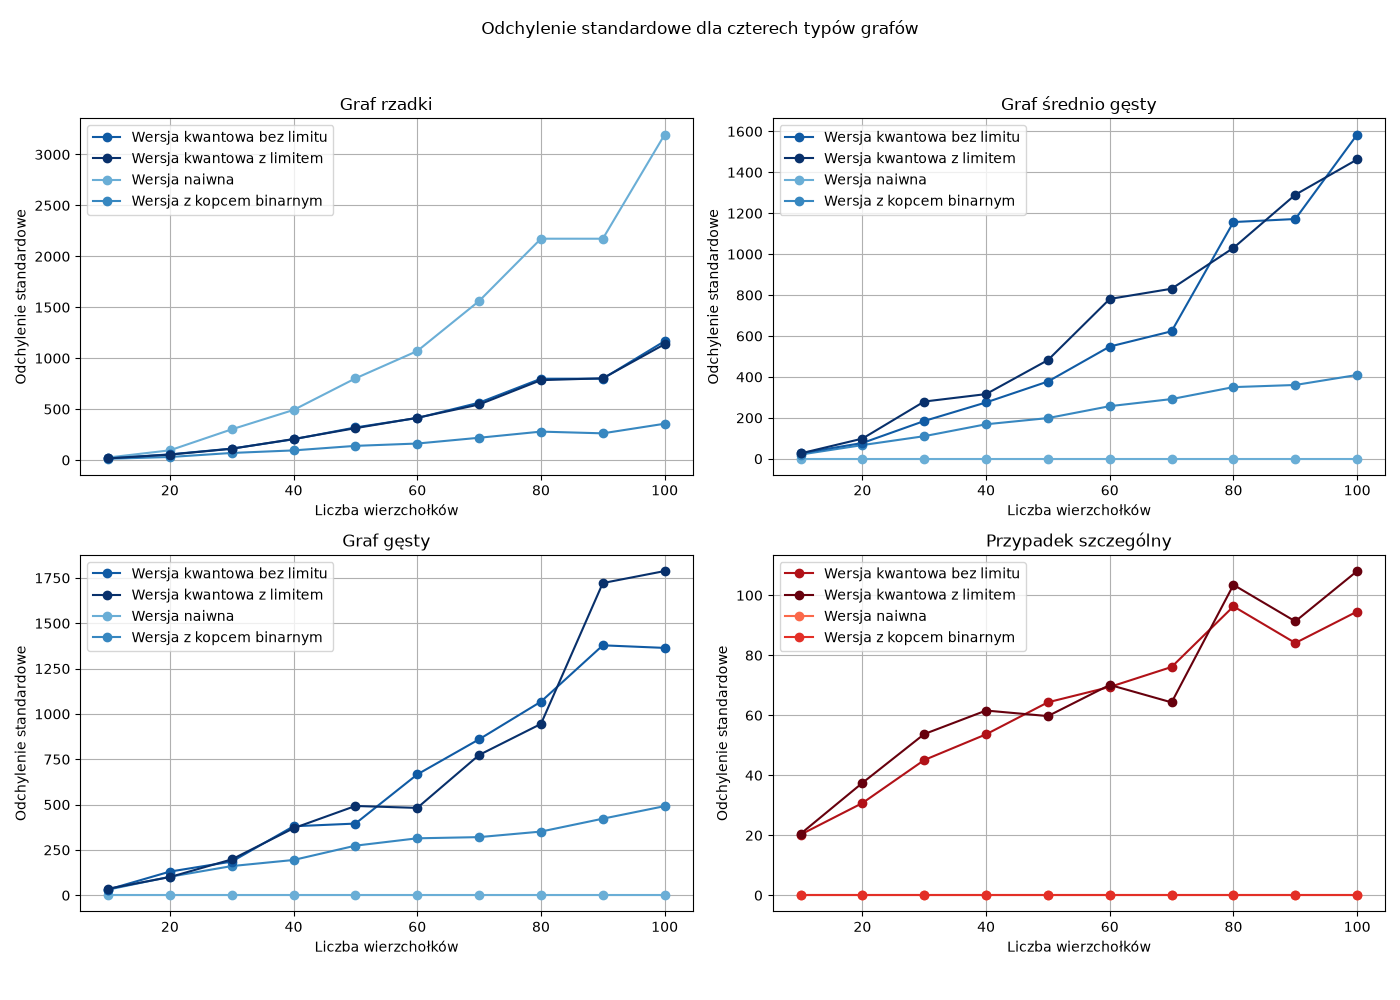
\includegraphics[width=\columnwidth]{images/documentation/combined/combined_std.png}
    \caption{Porównanie odchylenia standardowego liczby operacji wszystkich badanych implementacji dla czterech typów grafów.}
    \label{fig:combined_std}
\end{figure}

Rysunek~\ref{fig:combined_std} pokazuje, że poszczególne implementacje różnią się nie tylko średnim kosztem, ale też odchyleniem standardowym określającym jak stabilne są wyniki.

\subsection{Graf rzadki}

Dla grafów rzadkich szczególnie duże odchylenie standardowe występuje w wersji naiwnej. Jest ono spowodowane losową strukturą grafów oraz brakiem wymuszonej spójności. W zależności od wygenerowanego grafu algorytm może dotrzeć do dużej części wierzchołków albo zakończyć działanie znacznie wcześniej. To samo zjawisko zachodzi dla wersji z kopcem jednak w znacznie mniejszym stopniu. W przypadku implementacji kwantowej do zmienności spowodowanej strukturą grafu dochodzi probabilistyczny charakter BBHT i Dürra-Høyera. Powoduje to wzrost odchylenia standardowego wraz z rozmiarem grafu.

\subsection{Graf o średniej gęstości}

Dla grafów o średniej gęstości wersja naiwna jest bardzo stabilna, ponieważ dla tego rodzaju grafu algorytm Djikstry działa według tego samego schematu, nie ma problemu ze spójnością. Wersja z kopcem wykazuje większą zmienność, liczba operacji zależy od kolejności i liczby udanych relaksacji. Największy rozrzut średniej liczby operacji zauważalny jest dla implementacji kwantowych. Wynika to z losowej liczby prób BBHT i Dürra-Høyera. Wraz ze wzrostem liczby wierzchołków efekt ten staje się coraz bardziej widoczny.

\subsection{Graf gęsty}

Dla grafów gęstych utrzymuje się podobna zależność jak dla grafów o średniej gęstości. Wersja naiwna pozostaje bardzo stabilna, podczas gdy wyniki wersji z kopcem zależą od relaksacji. W implementacji kwantowej rozrzut tak jak dla grafów o średniej gęstości jest znacznie większy od implementacji klasycznych.

\subsection{Przypadek szczególny}

Przypadek szczególny pozwala dobrze rozdzielić wpływ struktury grafu na rozrzut wyników. Ze względu na specyficzny typ grafu odchylenie standardowe dla wersji klasycznych jest równe zeru niezależnie od liczby wierzchołków. Natomiast wersja kwantowa zachowuje niewielkie, lecz niezerowe odchylenie standardowe. Wynika ono z samego sposobu działania probabilistycznego wyszukiwania minimum. 
